% \addtocontents{toc}{\protect\newpage}
\chapter{Концептуальна модель та структура роботи}

\section{Мови програмування}
Мова програмування --- це індуктивний тип конструкторів мови,
для якої існує операційна семантка (правила обчислень) та правила виводу.
Найпростіша мова програмування --- нетипизоване лямбда числення,
ізоморфне екстракту в Erlang.

\section{Об'єкти}
Об'єкти категорій --- мови програмування. Кожна мова програмування
анонсує систему типів згідно свого індуктивного синтаксичного дерева.
Усі можливі екземпляри цього синтаксичного дерева є усіма
можливими программами в цій мові програмування.

\section{Мовні Категорії}
Мовна категорія --- це категорія, єдиний об’єкт якої це
синтаксичне дерево мови, а морфізми --- це стрілки
цієї maybe-категорії: [norm,type,infer,erase,extract]. Стрілки
зокрема містять правила виводу, типизації, нормалізації, екстактів, тощо.

\section{Вхідні синтаксиси. Специфікації}
Увесь спектр мов програмування, що сприймаються системою визначається набором
синтаксисів, парсери яких на виході дають індуктивні синтаксичні дерева
(закодовані у Бом, IR/II, чи будь-якому довільному індуктивному кодуванню).

\subsection{PTS синтаксиси}
Мінімальне ядро з однією аксіомою сприймає декілька лямбда ситаксисів.
Перший синтаксис сумісний з системою програмування
$morte$\footnote{http://github.com/Gabriel439/Haskell-Morte-Library}, та походить від неї.
Інший синтаксис сумісний з синтаксисом $cubical$\footnote{http://github.com/mortberg/cubicaltt}.
Планувалося також підтримати синтаксис $caramel$\footnote{https://github.com/MaiaVictor/caramel}.

\begin{lstlisting}[mathescape=true]
data PTS (A: U)
   = star (n: nat)
   | var (n: nat)
   | app (f a: A)
   | lambda (x: nat) (d c: A)
   | arrow (d c: A)
   | pi (x: nat) (d c: A)
\end{lstlisting}

\subsection{Індуктивні синтаксиси}
Індуктивні синтаксиси та кодування можуть підтримуватися за допомогою системи модулів.
Кожна система модулів може самостійно (у вигляді ефектів), або за допомогою лямбда кодувань
попередньої мови PTS рівня, зберігати та оперувати індуктивними типами даних.

Індуктивні синтаксиси будуються на телескопах Диб'єра,
конструкторах сум, та їх елімінаторах.

\begin{lstlisting}[mathescape=true]
data tele   (A: U) = nil | tel (n: name) (b: A) (xs: tele A)
data branch (A: U) =        br (n: name) (a: list name) (t: A)
data label  (A: U) =       lab (n: name) (t: tele A)

data Inductive (A: U)
   = parent (p: PTS (Inductive A))
   | sum  (n: name) (t: tele A) (labels:   list (label A))
   | case (n: name) (t: ind)    (branches: list (branch A))
   | ctor (n: name)             (args:     list A)
\end{lstlisting}

\subsection{Інші синтаксиси та мови}
Система не повинна бути обмежена мовами та синтаксисами, ми покажемо як приклад,
підтримку гомотопічної мови з інтервалом [0,1] сумісної з $cubical$ та з пітримкою індуктивних
синтаксисів та кодувань попереднього рівня.

\begin{lstlisting}[mathescape=true]
data alg
   = zero
   | one
   | max (a b: alg)
   | min (a b: alg)

data HTS (A: U)
   = parent (p: Inductive (HTS A))
   | path (a b: A)
   | pathLam (n: nat) (a b: A)
   | pathApp (f: alg) (a b: A)
   | comp (a b: A)
   | fill (a b c: A)
   | glue (a b c: A)
   | glueElem (a b: A)
   | unglueElem (a b: A)
\end{lstlisting}

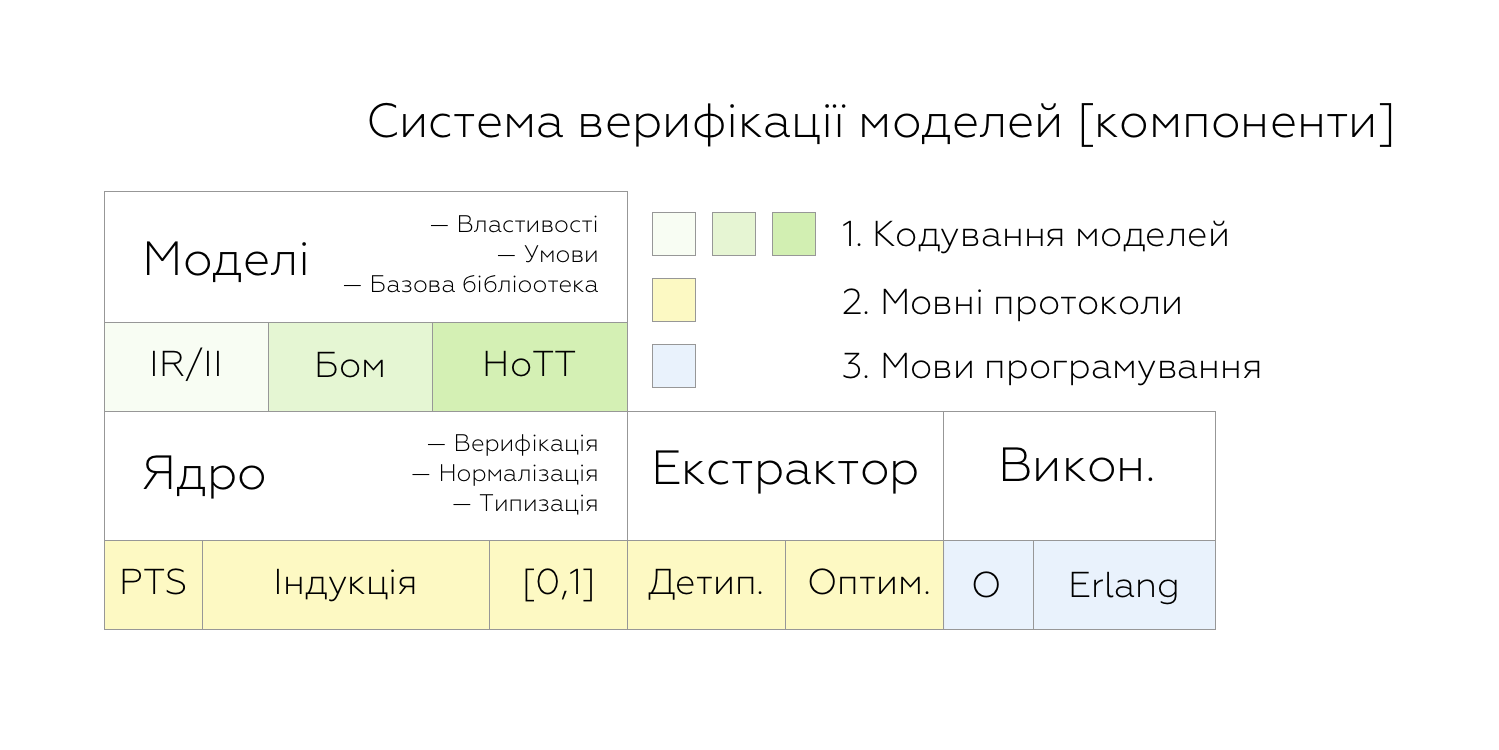
\includegraphics[scale=0.18]{static}

\section{Вихідні синтаксиси. Екстракт}
Кількість мов прототипа обмежена двома інтерпретаторами: O та Erlang,
однак система не обмежується цими мовами, а має експериментальне HM ядро
з екстрактом в С++. Цікаво було би отримати екстракт в Rust.

\begin{lstlisting}[mathescape=true]
data O
   = var (n: nat)
   | app (f a: O)
   | lambda (x: nat) (d c: O)
\end{lstlisting}

Вхідними синтаксисами екстраторів є синтаксиси відповідної мови ядра.
На даний момент в роботі ми підтримуємо PTS та індуктивний синтаксиси.

\section{Динаміка. Морфізми}

Кожна мова програмування може бути доменом або кодоменом
морфізмів в категорії мов програмування. На малюнку зображена
композиція морфізмів (верифікації та екстрагування)
в maybe-категорії (побудованої maybe функтором) у вигляді BPMN процесу.

\begin{lstlisting}[mathescape=true]
process (p: maybe PTS): maybe Erlang
  = extract1 (erase (opt (norm (type p))))
\end{lstlisting}

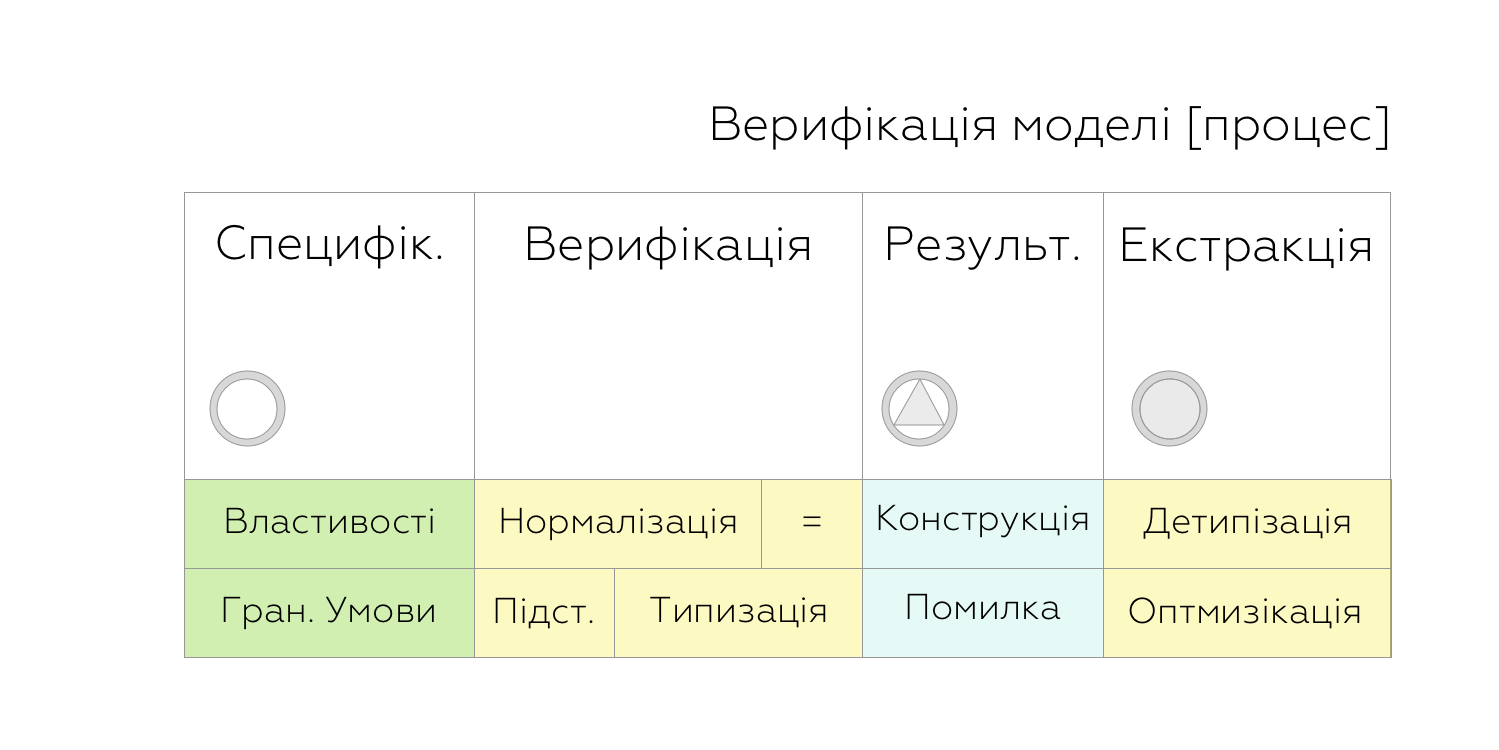
\includegraphics[scale=0.18]{dynamic}

\begin{lstlisting}[mathescape=true]
type (A: maybe PTS): maybe PTS
norm (A: maybe PTS): maybe PTS
erase (A: maybe PTS): maybe ULC
opt (A: maybe PTS): maybe PTS
extract1 (A: maybe ULC): maybe Erlang
extract2 (A: maybe ULC): maybe O
extract3 (A: maybe ULC): maybe C++
extract4 (A: maybe Inductive): maybe Erlang
\end{lstlisting}

Функторіальні мовні перетворення: 1) extract: maybe A -> maybe B --- з однієї
мови програмування А в іншу мову програмування B; 2) type: maybe A -> maybe A
--- перевірка терма первної мови програмування; 3) infer: maybe A -> maybe A
--- типізація; 4) norm: maybe A -> maybe A --- нормалізація.

% \newpage
% \section{Формалізація концепції}

\begin{center}
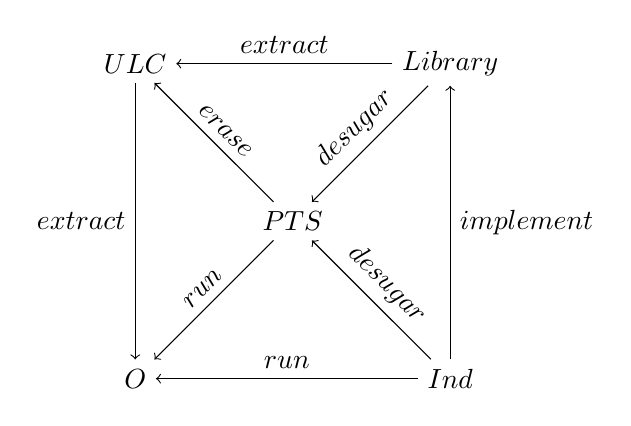
\begin{tikzpicture}
\tikzstyle{every initial by arrow}=[]
    \node (a) at (0,0) {$O$};
    \node (b) at (0,4) {$ULC$};
    \node (c) at (4,0) {$Ind$};
    \node (d) at (4,4) {$Library$};
    \node (e) at (2,2) {$PTS$};
    \draw [->] (b) to node [left] {$extract$} (a);
    \draw [->] (c) to node [above] {$run$} (a);
    \draw [->] (e) to node [above,sloped] {$run$} (a);
    \draw [->] (d) to node [above,sloped] {$desugar$} (e);
    \draw [->] (d) to node [above] {$extract$} (b);
    \draw [->] (e) to node [above,sloped] {$erase$} (b);
    \draw [->] (c) to node [above,sloped] {$desugar$} (e);
    \draw [->] (c) to node [right] {$implement$} (d);
\end{tikzpicture}
\end{center}

\begin{fullwidth}
\hspace{0cm}
\begin{tabular}{lll}
  $PTS: cat(PTS,hom)$ &---& PTS категорія \\
  $Ind: cat(Inductive,hom)$ &---& Індуктивна категорія \\
  $Library: Inductive$ &---& Базова бібліотека як програма Індиктивної мови\\
  $desugar: Ind \rightarrow PTS$ &---& Сам прувер є розширенням ядра \\
  $implement: Ind \rightarrow Library$ &---& Базова біблотека написана на Індуктивній мові \\
  $lower: Ind \rightarrow PTS$ &---& Базова бібліотека конвертується в код ядра \\
  $erase: PTS \rightarrow ULC$ &---& Видаляється інформація про типи, детипізація \\
  $extract: ULC \rightarrow O$ &---& Запуск на інтерпритаторі \\
\end{tabular}
\end{fullwidth}

\section{Операційні семантики}
\section{Мови та Мовні рівні}

\begin{lstlisting}
System F-omega
Kind κ = * | κ → κ | ···
Con c  =
       | arr(c₁; c₂) c₁ → c₂        (Con, Con) Con
       | all {κ} (u.c) ∀ (u ∷ κ). c (Kind, Con.Con) Con
       | lam {κ} (u.c) λ (u ∷ κ). c (Kind, Con.Con) Con
       | app(c₁; c₂) c₁ (c₂)        (Con, Con) Con
\end{lstlisting}

\section{Середовище виконання (ОС)}
\section{Специфікації мов}
\section{Властивості}
\section{Нормалізація та оптимізація}
\section{Екстракція}
\section{Обмеження}
\section{Область застосування}

